% \documentclass{article}
% % \usepackage[utf8]{inputenc}
% \usepackage{fullpage}
% \usepackage {setspace}
% \usepackage[hang,flushmargin]{footmisc} %control footnote indent
% \usepackage{url} % for website links
% \usepackage{amssymb,amsmath}%for matrix
% \usepackage{graphicx}%for figure
% \usepackage{appendix}%for appendix
% \usepackage{float}
% \usepackage{multirow}
% \usepackage{longtable}
% \usepackage{morefloats}%in case there are too many float tables and figures
% \usepackage{caption}
% \usepackage{subcaption}
% \usepackage{listings}
% \captionsetup[subtable]{font=normal}
% \usepackage{color}
% \usepackage{hyperref}
% \usepackage[round]{natbib}
% \usepackage[export]{adjustbox}
% %\usepackage{Sweave}
% \setlength{\parindent}{0em}
% \setlength{\parskip}{0.5em}


% \graphicspath{{0.plots/}}


% \begin{document}
\subsection{Application}\label{sec:p2data}
\subsubsection{The Atherosclerosis Risk in Communities (ARIC) Study}\label{sec:p2data_analysis}
%%%% briefly talk about which data will be used then talk about clinical background of HD
We apply the proposed QRJM to the data derived from the Atherosclerosis Risk in Communities Study (ARIC). ARIC is a prospective epidemiological study conducted in four diverse U.S. communities (i.e. Forsyth County in North Carolina, Jackson County in Mississippi, Minneapolis suburbs in Minnesota, and Washington County in Maryland). The aims of ARIC are to investigate the causes of atherosclerosis and its clinical outcomes, and variation in cardiovascular risk factors, medical care, and disease by race, gender, location, and date \citep{aric1989atherosclerosis}. In the ARIC cohort study component, a cohort sample of approximately 4000 individuals aged 45 $-$ 64 years were randomly selected from each of the four ARIC field centers as the representatives of the community to receive extensive follow-up study. The cohort recruitment was started in 1987 and the first screening examination was conducted in 1987 $-$ 1989 when the baseline data were collected. Additional three cohort follow-up examinations were conducted at approximately three-year intervals, in 1990 $-$ 1992, 1993 $-$ 1995, and 1996 $-$ 1998, when the longitudinal measures were created. Follow-up also occurs semi-annually, by telephone, to maintain contact and to assess health status of the cohort.

%%%% More details on the ARIC study and the data set: longitudinal part and time-to-event part
One of the objectives of the cohort study is to investigate the trends in rates of hospitalized myocardial infarction (MI) and coronary heart diseases (CHD) in those communities. It is reported in previous studies of ARIC data that risk factors for CHD differ significantly by race group. \cite{wattanakit2005risk, rodriguez2014systolic} also showed that systolic blood pressure (SBP) was an important risk factor for CHD events in the ARIC cohort. However, few studies have considered the time change rate of SBP among hypertensive patients, especially the time effect on different quantiles of SBP, and its association with the risk of recurrent CHD events. To fill the gap, we aim to use the proposed QRJM to investigate the baseline covariate effects and time change rate on different quantiles of SBP and to characterize the association between SBP trajectory and recurrence of CHD events.

Data used in this study is derived from one of the four study communities, in which we include only white hypertensive participants (with SBP $>$ 140 mm Hg and DBP $>$ 90 mm Hg at baseline or self-reported history of physician-diagnosed hypertension or taking anti-hypertensive medicine). Participants who had prevalent CHD (defined by Q waves on the electrocardiogram, self-reported history of MI diagnosis, coronary artery bypass graft, or coronary angioplasty) before the first examination are excluded from the analysis. The resulting study cohort consists of 657 participants. Repeated measures of SBP were collected from the four longitudinal examination cycles that started at 1987 and ended at 1998. Out of the total 657 participants, 440 (67\%) individuals had four complete SBP measures, 113 (17\%), 54 (8\%), and 50 (8\%) had three, two and only one measure respectively. The LOESS curve in Figure ~\ref{fig:p2_sbp_loess} shows no obvious time trend for SBP in approximately 11-year follow-up period. Follow-up for recurrent CHD events continued through 2010. The median follow-up time is 21 years with the maximum as 24 years. 242 (36\%) deaths occurred during the follow-up and 115, 31, and 17 patients experienced one, two or more than two CHD events. Baseline characteristics of the study cohort is presented in Appendices Table ~\ref{tab:p2cht_baseline}.

\begin{figure}[H]
\centering
% 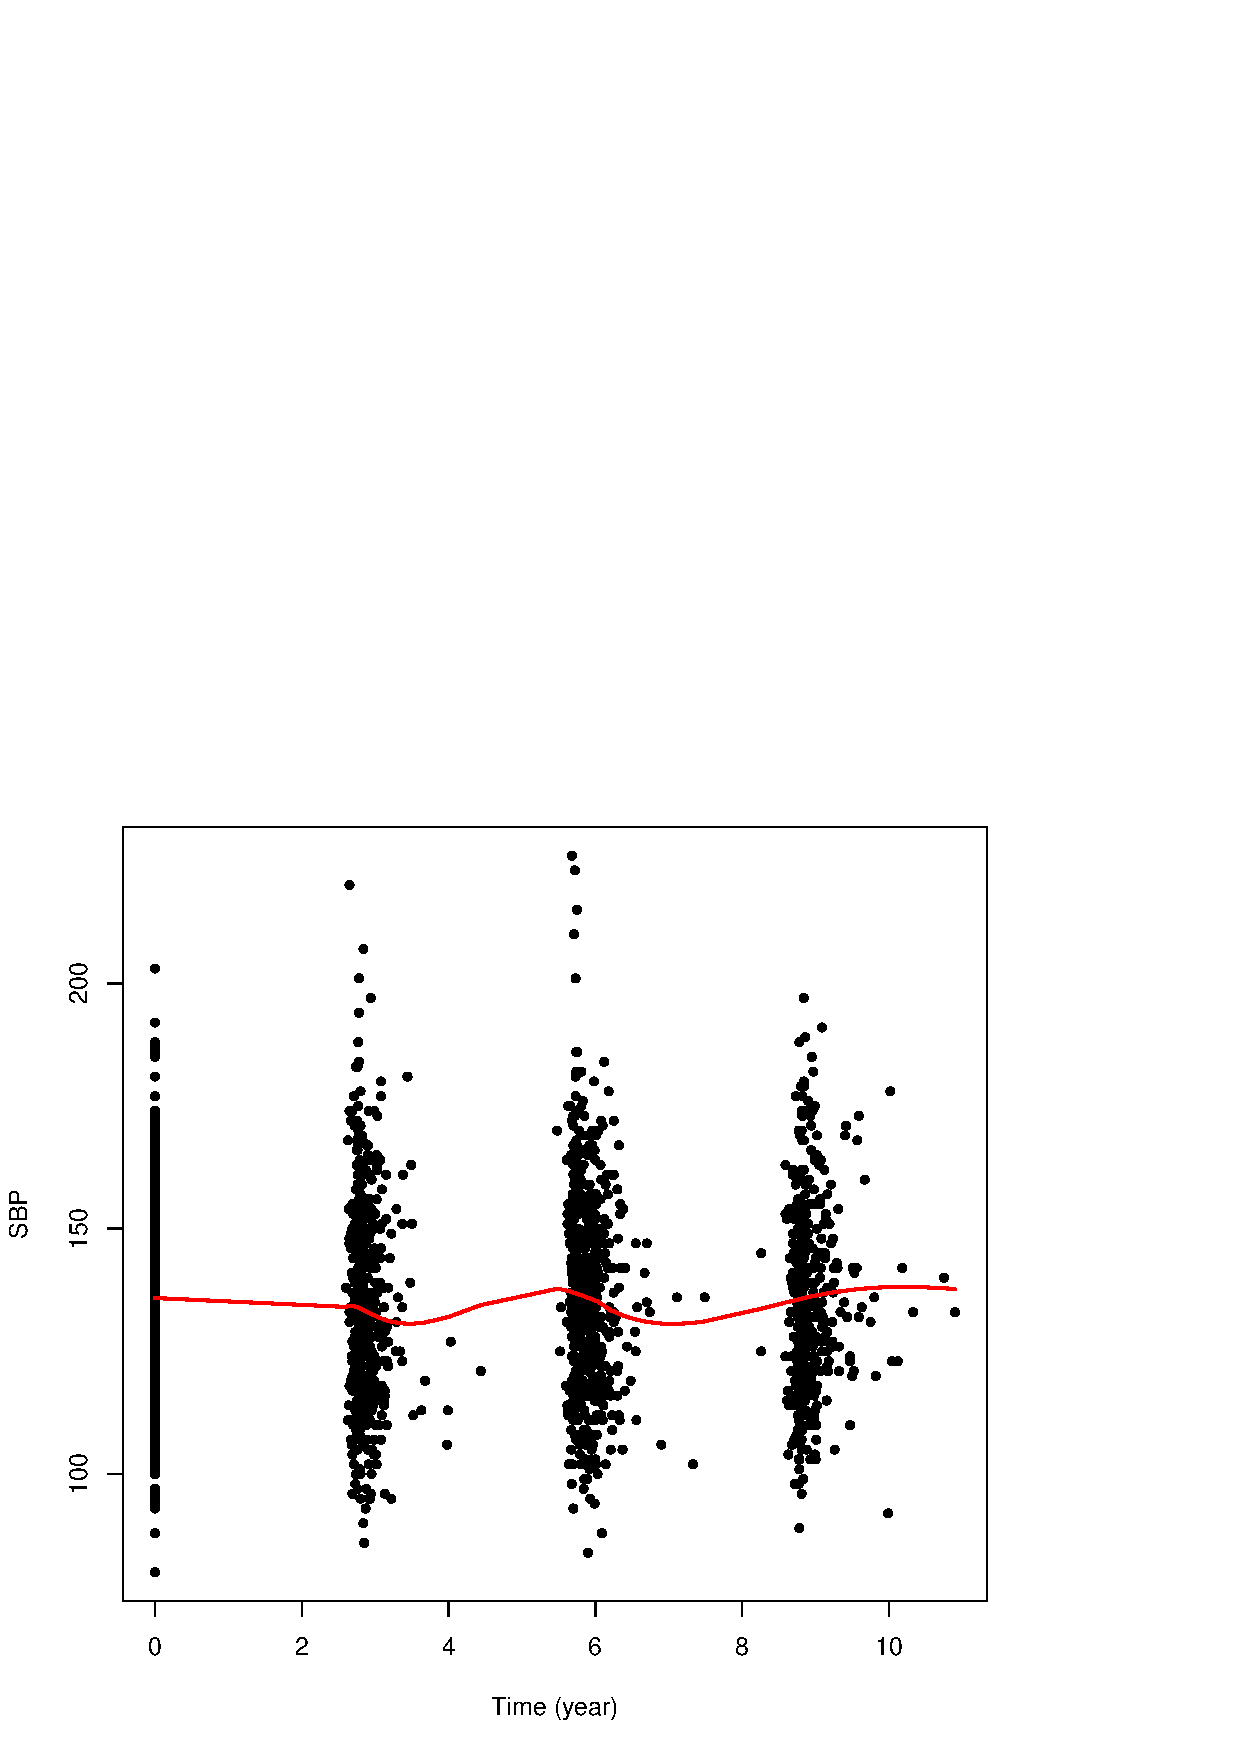
\includegraphics[width=\columnwidth]{SBP_loess.pdf}
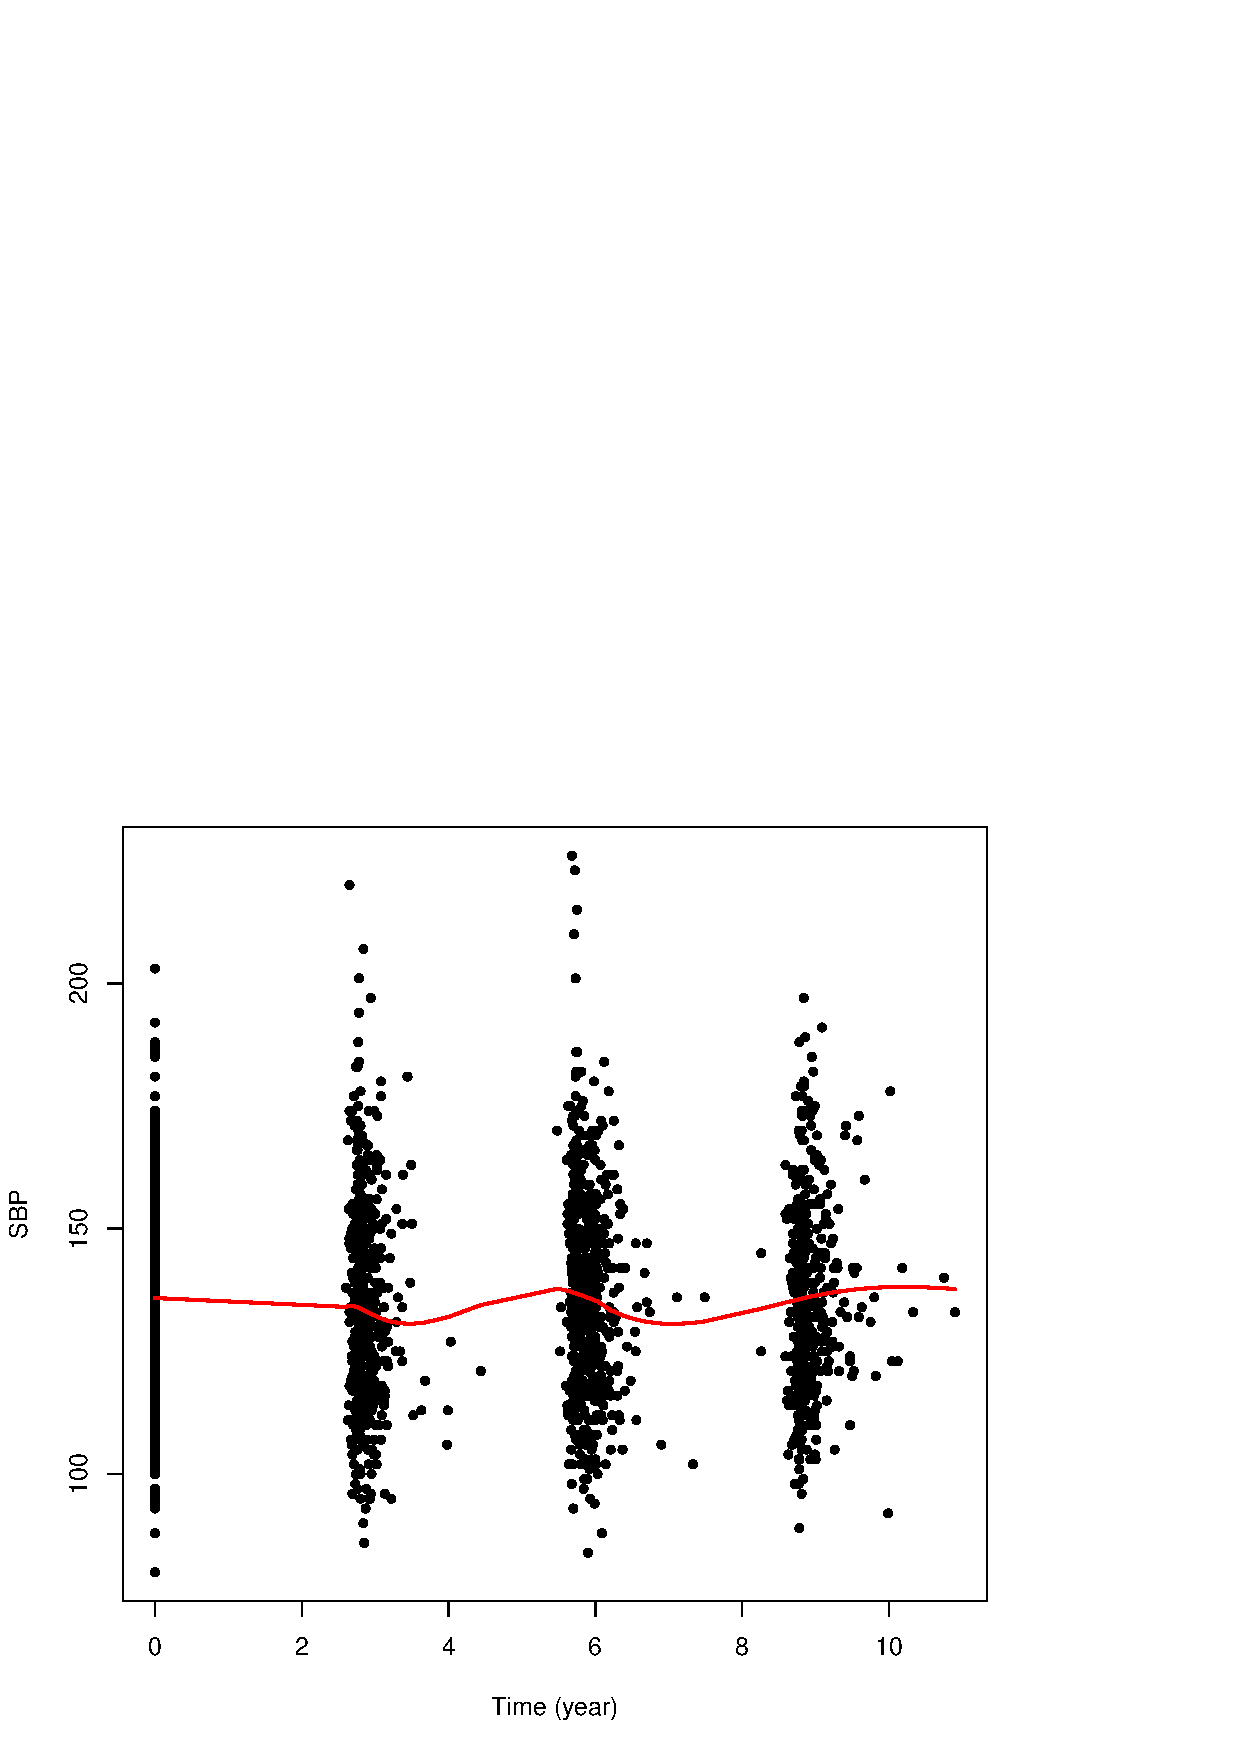
\includegraphics[scale=0.6]{SBP_loess.pdf}
\caption{Scatter plot with LOESS curve of longitudinal SBP measures in the study cohort.}
\label{fig:p2_sbp_loess}
\end{figure}

In data analysis, follow-up time is converted from days to years and the first examination date is set to time 0; baseline age is centered by subtracting the overall mean, and total-cholesterol is standardized to have mean 0 and standard deviation 1. We consider the following QRJM:
\small{
\begin{equation*}\label{eqn:p2data_joint}
\left\{
\begin{array}{l}
sbp_{i}(t) = m_{i}(t) + \varepsilon_{i}(t) = \beta_0 + \beta_1 age_{0i} + \beta_2 chol_i + \beta_3 I_{hyper-med_i}+ \beta_4 t + {u}_{i1} + u_{i2} t + \varepsilon_{i}(t)\\
r_i(t|\mathcal{M}_{it};  \boldsymbol{\gamma}, \alpha) = \sum_{k=1}^3v_i\lambda_kI_k(t)\exp(\gamma_1 I_{male_i} + \gamma_3 I_{smoke_i} + \gamma_4I_{diabetes_i} + \alpha m_i(t))
\end{array}
\right.
\end{equation*}
}
where we assume  $\varepsilon_{i}(t)\sim ALD(0, \sigma, \tau)$. $age_0$ is the baseline age at the first examination, $chol$ stands for the total-cholesterol level (mg/dL), $I_{hyper-med}$ is the variable indicating whether an individual had taken hypertension lowering medication, $t$ is the follow-up time, and $u_{i1}$ and $u_{i2}$ are subject-specific random intercept and slope to account for the within subject correlation and between subject variation. In the recurrent event submodel, we specify a piecewise constant baseline intensity function with three time intervals, where $\lambda_k$ is the hazard rate for time interval $[t_{k-1}, t_{k})$, that is $I_k(t)=1$ if $t\in[t_{k-1}, t_{k})$ and 0 otherwise. Knots $t_1$ and $t_2$, used to define piecewise constant time intervals, are selected as the 33.3\% and 66.7\% percentiles of the ordered follow-up time; while $t_0$ = 0 and $t_3$ is the maximum of follow-up time. We also include a frailty term $v_i$ in the recurrent event model that introduces correlation of multiple CHD events within the same individual. Other model covariates include indicator variables for male ($I_{male}$), ever smoke ($I_{smoke}$), and diabetes mellitus ($I_{diabetes}$). In the QRJM, the true underlying longitudinal measure of SBP is treated as a time dependent covariate in the recurrent event process and $\alpha$ is the association parameter governing the dependence between these two processes. Two chains with diverse initial values are initiated in the Bayesian inference algorithm and the chains are considered to converge if the potential scale reduction factors (PSRF) for all parameters are below 1.1.


\subsubsection{Inference Results for ARIC data}\label{sec:p2data_results}
Inference results from five different quantiles (0.05, 0.25, 0.50, 0.75, and 0.95) of SBP are shown in Table~\ref{p2realdata_inference} as well as visualized in Figure~\ref{p2_jm_infer}. In the longitudinal SBP process, older participants generally have higher SBP level and the effect of baseline age is consistently positive across all five selected quantiles of SBP. For example, one year increase in baseline age is associated with 0.037 (95\% CI: (0.028, 0.047)) unit increase in the median (i.e., $\tau=0.50$) of standardized SBP in the study cohort when controlling for other covariates. Total cholesterol level is negatively associated with SBP; however, the effects are not significant across all five quantiles. In general, people who took hypertension medications have significantly lower SBP and the effect of taking hypertension medications is larger at higher levels of SBP. Moreover, it is interesting to see that follow-up time has a significantly positive effect on higher quantiles of SBP (i.e., $\tau=0.75$ and 0.95) while for lower quantiles ($\tau=0.05$, 0.25, and 0.50) the effect is not significant. This finding can be an important indication that among the hypertension patients who originally have excessively higher SBP deteriorate even faster than those with lower SBP.

In the recurrent CHD event process, we see all positive association between the five conditional quantiles of SBP and the risk of CHD event, which coincide with our expectation as well as previous findings from ARIC data. However, the degree of association between these two processes varies among the conditional quantiles and is found to be strongest at the conditional median of SBP (relative risk:1.25, 95\% CI: (1.02, 1.53)) among the five selected quantiles. For other regression covariates, diabetic patients are at significantly higher risk of having recurrent CHD event compared with non-diabetic. For example, when controlling for other factors, the risk of having additional CHD event is 2.3 times higher ($\exp(0.85)$, 95\% CI: (1.46, 3.85)) for people with diabetes than those who are free of the disease at $\tau=0.5$. We also observed the posterior effect of diabetes decreases as quantile increases. This indicates that the effect of diabetes on the risk of recurrent CHD event is less important for patients with higher SPB. Although  male patients and ever smokers are also at higher risk of experiencing CHD events, the relative risks are statistically insignificant compared with female and never smokers respectively.

\newpage
\thispagestyle{lscape}
\pagestyle{lscape}
\begin{landscape}
\doublespacing
% \begin{sidewaystable}[H]
\begin{table}[H]
\centering
\caption{ARIC data analysis: Parameter estimation and 95\% credible interval (in parenthesis) from QRJM at five quantiles.}
\label{p2realdata_inference}
\resizebox{\linewidth}{!}{
\begin{tabular}{lccccc}
  \hline
  & $\tau=0.05$ & $\tau=0.25$ & $\tau=0.50$ & $\tau=0.75$ & $\tau=0.95$\\
\hline
\multicolumn{6}{c}{\textit{longitudinal SBP process}}  \\
  intercept & -0.374 (-0.478, -0.274) & -0.023 (-0.118, 0.074) & 0.447 (0.352, 0.554) & 0.872 (0.775, 0.978) &1.187 (1.079, 1.300)\\
  age$_0$ & 0.035 (0.026, 0.044) & 0.034 (0.025, 0.044) & 0.037 (0.028, 0.047) & 0.040 (0.030, 0.050) & 0.043 (0.031, 0.052)\\
  total-chol.(mg/dL) & -0.020 (-0.073, 0.033) & -0.026 (-0.081, 0.032) & -0.022 (-0.078, 0.037) & -0.013 (-0.073, 0.047) & -0.022 (-0.076, 0.032)\\
  hypertension medicine & -0.583 (-0.710, -0.467) & -0.652 (-0.773, -0.538) & -0.725 (-0.842, -0.609) & -0.730 (-0.868, -0.593) & -0.787 (-0.924, -0.660)\\
  follow-up time (yr) & 0.008 (-0.003, 0.018) & 0.006 (-0.006, 0.019) & 0.011 (-0.001, 0.022) & 0.016 (0.004, 0.029) & 0.019 (0.005, 0.033)\\
  \multicolumn{6}{c}{\textit{recurrent CHD event process}}  \\
  association & 0.163 (-0.003, 0.332) & 0.207 (0.011, 0.405) & 0.226 (0.019, 0.428) &  0.205 (0.034, 0.374) &0.162 (0.028, 0.288)\\
  male & 0.191 (-0.152, 0.548) & 0.185 (-0.170, 0.528) &  0.160 (-0.187, 0.507) & 0.132 (-0.205, 0.477) & 0.110 (-0.234, 0.458)\\
  ever  smoke & 0.291 (-0.044, 0.641) & 0.271 (-0.070, 0.613) & 0.216 (-0.121, 0.552) & 0.165 (-0.177, 0.493) & 0.163 (-0.184, 0.485)\\
  diabetes & 0.918 (0.424, 1.399) & 0.895 (0.409, 1.376) & 0.850 (0.381, 1.349) & 0.811 (0.352, 1.318) & 0.818 (0.333, 1.301)\\
  $\lambda_1$ & 0.011 (0.010, 0.013) & 0.011 (0.010, 0.013) & 0.011 (0.010, 0.012) & 0.011 (0.010, 0.012) & 0.011 (0.010, 0.012)\\
  $\lambda_2$ & 0.028 (0.020, 0.036) & 0.027 (0.019, 0.035) & 0.026 (0.018, 0.034) & 0.024 (0.017, 0.032) & 0.024 (0.017, 0.032)\\
  $\lambda_3$ & 0.073 (0.037, 0.113) & 0.072 (0.036, 0.111) & 0.067 (0.034, 0.105) & 0.065 (0.033, 0.103) & 0.066 (0.034, 0.103)\\
   \hline
\end{tabular}
}
\end{table}
% \end{sidewaystable}
\end{landscape}

\restoregeometry
\pagestyle{plain}

\newpage
\begin{figure}[H]
\centering
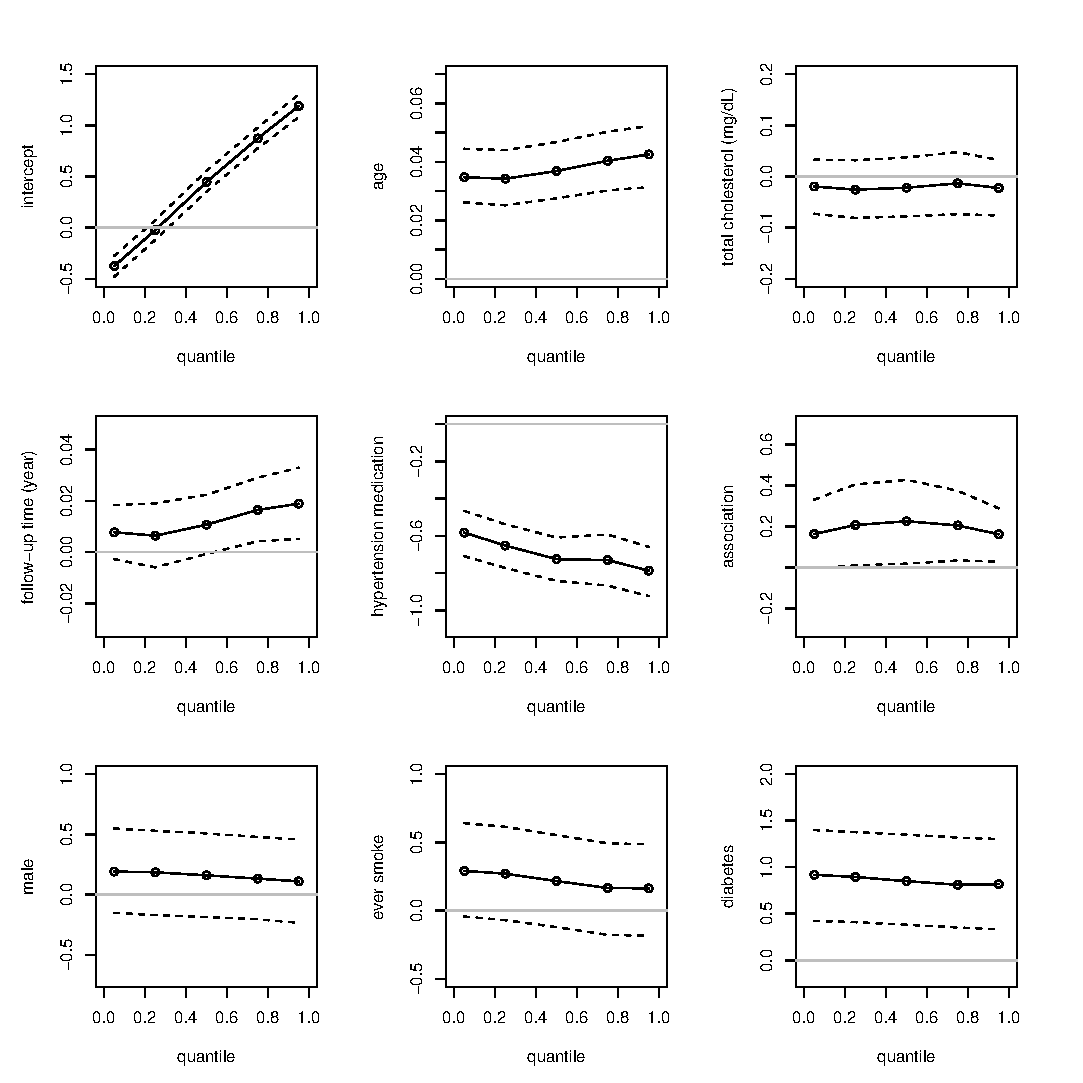
\includegraphics[width=\textwidth]{0.plots/p2_JM_inference_covs.eps}
\caption{ARIC data analysis: Posterior mean (solid line) and point-wise 95\% credible interval (dashed lines) of parameter estimation against different quantiles.}
\label{p2_jm_infer}
\end{figure}




% \end{document}
